\documentclass[11pt,evaluacion]{uescimat}

\usepackage[utf8]{inputenc} % utilice "latin1" si 
\usepackage{multienum}
\usepackage{multicol}
\usepackage{enumerate}
\usepackage{enumitem}
\usepackage{float}


\usepackage[spanish]{babel}
 
\addto\captionsspanish{
\def\tablename{Tabla}
\def\listtablename{\'Indice de tablas}
}



\materia{Estadística I}
\ciclo{II}
\anoacademico{2017}
%\fecha{Jueves 23 de Marzo de 2017}
\titulo{Guía de ejercicios Unidad \#2}

\begin{document}

%\setlist{nolistsep}   % si lo que queremos es que no haya espacios


\setlist[enumerate]{itemsep=0mm}

\maketitle

%{ \scriptsize

%\begin{indicaciones}

%\end{indicaciones}

\begin{problema}
La siguiente tabla de contingencia son de estudiantes de estadística I en la Universidad de Adelaida. A los cuales se les pregunto si fumaban (filas) y si realizaban ejercicio físico (columnas). Se pide analizar estos datos para ver si existe asociación entre fumar y realizar ejercicio físico. Se incluye el gráfico de barras apilado y el gráfico de mosaico. 

\begin{table}[H]
\centering
\begin{tabular}{rrrr}
\hline 
& & \textbf{Hace Ejercicio} & \\
  \hline
\textbf{Fuma} & Algo & Frecuentemente & Ninguno \\ 
  \hline
Mucho &   3 &   7 &   1 \\ 
  Nunca &  84 &  87 &  18 \\ 
  Ocasionalmente &   4 &  12 &   3 \\ 
  Regularmente &   7 &   9 &   1 \\ 
   \hline
\end{tabular}
\end{table}


\begin{figure}[H]
\begin{centering}
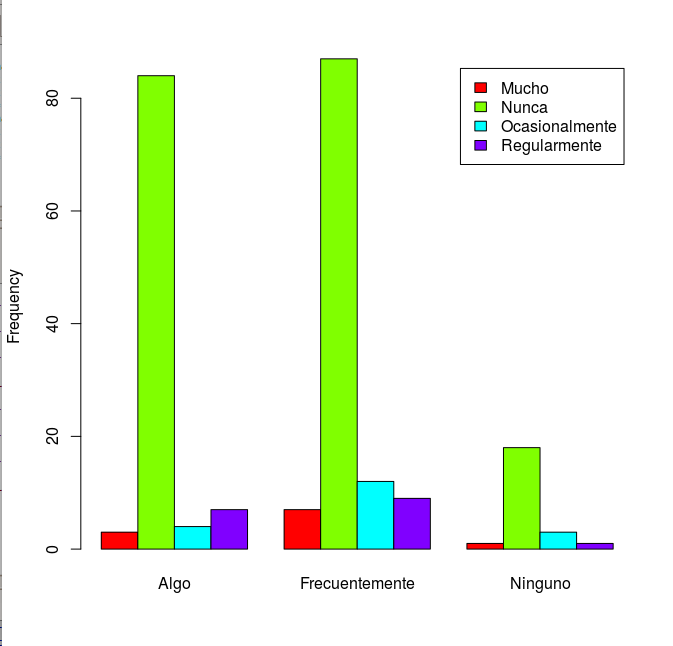
\includegraphics[scale=0.30]{imagen1.png}
\par\end{centering}
\caption{Fumar versus hacer ejercicio}

\end{figure}


\begin{figure}[H]
\begin{centering}
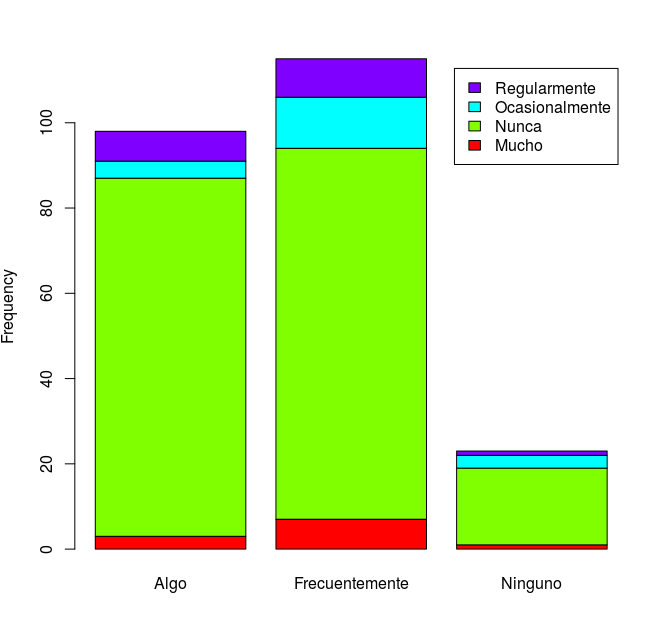
\includegraphics[scale=0.30]{imagen2.png}
\par\end{centering}
\caption{Fumar versus hacer ejercicio}

\end{figure}



\end{problema}


\begin{problema}
En un estudio de Senie et al. (1981) se investiga la relación entre la edad y la frecuencia de examinación de auto-examen para detectar el cancer de seno en una muestra de mujeres. A continuación se presenta la tabla de contingencia, el gráfico de barras agrupado y el gráfico de mosaico. Se pide analizar estos resultados y mencionar como estan asociadas las dos variables. 

\begin{table}[H]
\centering
\begin{tabular}{rrrr}
\hline 
 & & \textbf{Frecuencia de auto-examinación} & \\
  \hline
\textbf{Edad} & Mensualmente & Ocasionalmente & Nunca \\ 
  \hline
Abajo de 45 &   91 &   90 &   51 \\ 
Entre 45 - 59 &  150 &  200 &  155 \\ 
60 y más  &   109 &  198 &   172 \\ 
   \hline
\end{tabular}
\end{table}


\begin{figure}[H]
\begin{centering}
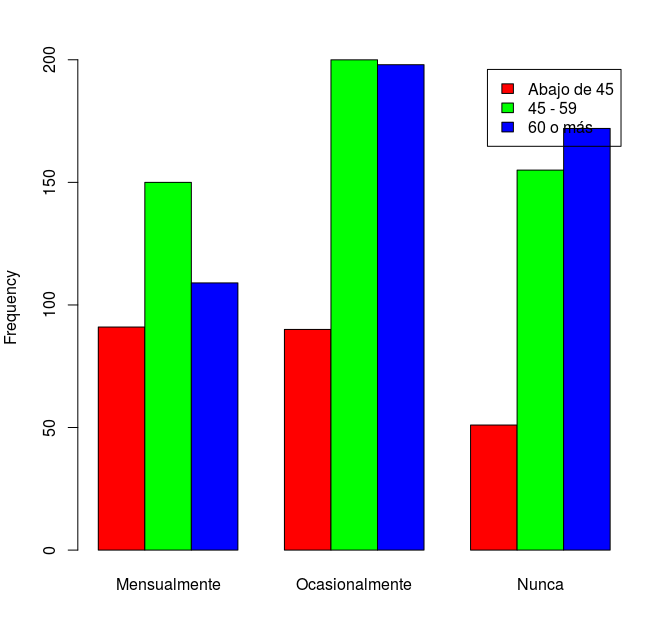
\includegraphics[scale=0.30]{imagen3.png}
\par\end{centering}
\caption{Edad versus frecuencia de autoexamen}
\end{figure}

\begin{figure}[H]
\begin{centering}
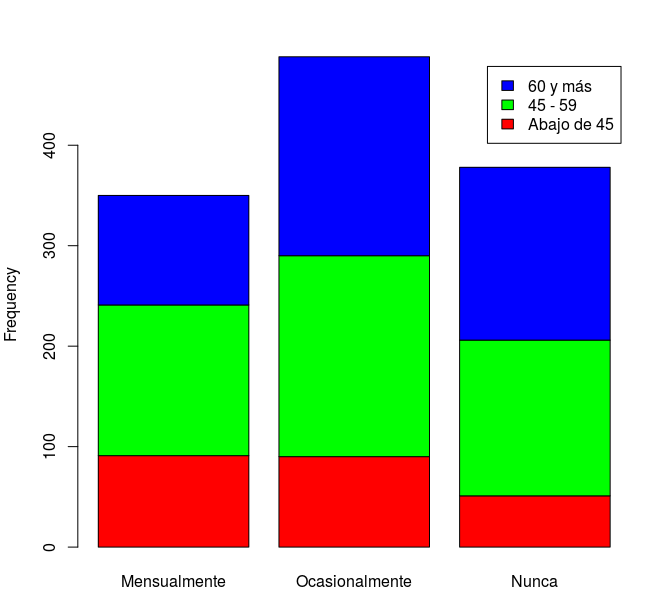
\includegraphics[scale=0.30]{imagen4.png}
\par\end{centering}
\caption{Edad versus frecuencia de autoexamen}
\end{figure}




\end{problema}


\begin{problema}
En los siguientes gráficos se presentan el gráfico de cajas y el histograma de la tasa de mortalidad de cancer de melanoma (cancer de piel) en los estados de USA segmentado por la variable oceano la cual representa cercania al océano (yes) o lejania (no). Se pide analizar la asociación entre el cancer de piel y cercania al oceano. Analize si son adecuados los gráficos de cajas.

\begin{figure}[H]
\begin{centering}
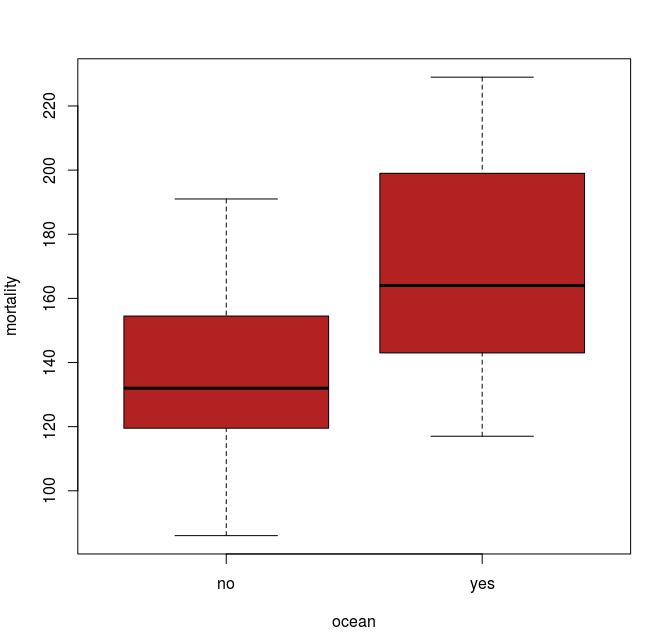
\includegraphics[scale=0.30]{imagen5.png}
\par\end{centering}
\caption{Tasa de mortalidad de cancer de piel versus cercania al oceano}
\end{figure}

\begin{figure}[H]
\begin{centering}
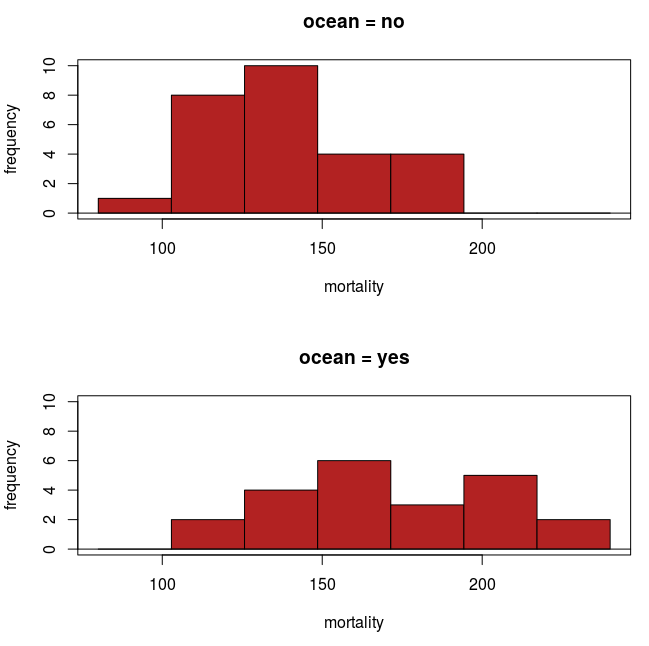
\includegraphics[scale=0.30]{imagen6.png}
\par\end{centering}
\caption{Tasa de mortalidad de cancer de piel versus cercania al oceano}
\end{figure}



\end{problema}


\begin{problema}
En los siguientes gráficos se muestra datos de calificaciones de notas en matemáticas en dos grupos de 40 alumnos en un colegio. Que puedo decir de los resultados de las notas en las dos secciones. Analize si son adecuados los gráficos de cajas. 


\begin{figure}[H]
\begin{centering}
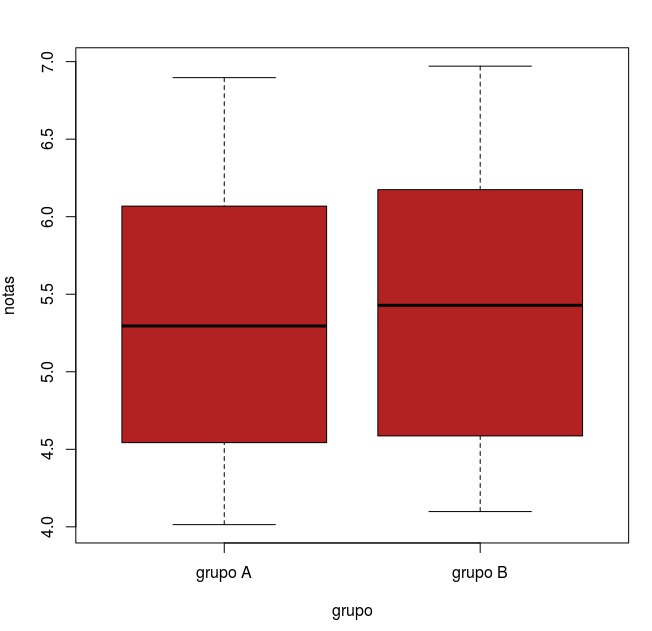
\includegraphics[scale=0.30]{imagen7.png}
\par\end{centering}
\caption{Notas en grupos}
\end{figure}

\begin{figure}[H]
\begin{centering}
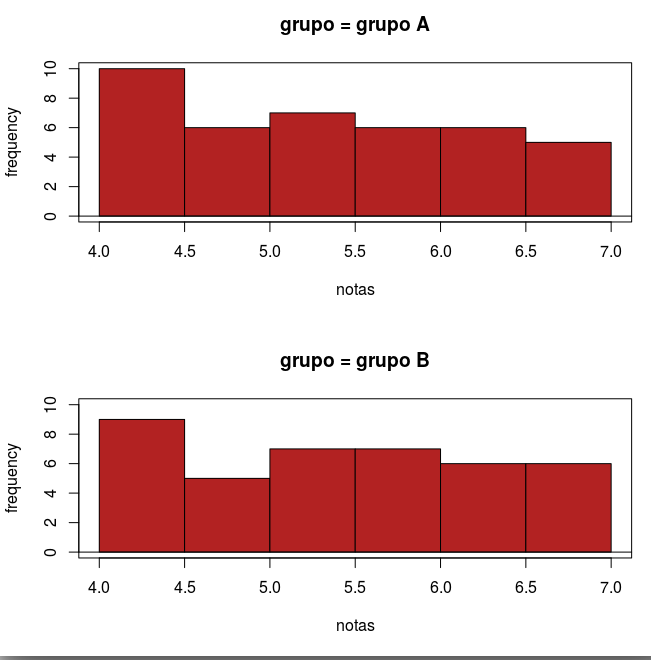
\includegraphics[scale=0.30]{imagen8.png}
\par\end{centering}
\caption{Notas en grupos}
\end{figure}


\end{problema}


\begin{problema}
En cada una de las situaciones siguientes, ¿qué es más razonable, simplemente explorar la relación entre dos variables o contemplar una de las variables como
variable explicativa y la otra como variable respuesta?

\begin{enumerate}[label=(\alph*)]
\item La cantidad de tiempo que un alumno pasa estudiando para un examen
de Estadística y la calificación obtenida en el examen.
\item El peso y la altura de una persona.
\item La lluvia caída durante un año y el rendimiento de un cultivo.
\item Las calificaciones de Estadística y de Francés de los estudiantes.
\item El tipo de trabajo de un padre y el de su hijo.
\end{enumerate}



\end{problema}


\begin{problema}
¿Es posible predecir la altura que tiene un niño de 16 años a partir de la altura que tenía a los 6? Una manera de descubrirlo consistiría en medir la altura
de un grupo suficientemente numeroso de niños de 6 años, esperar hasta que
cumplieran los 16 años y entonces volver a medirlos. En este caso, ¿cuál es la variable explicativa y cuál es la variable respuesta? ¿Estas variables son categóricas
o cuantitativas?
\end{problema}

\begin{problema}
El inventor de un nuevo material aislante quiere determinar
la magnitud de la compresión que se producirá en una pieza de 2 pulgadas
de espesor cuando se somete a diferentes cantidades de presión. Para ello
prueba 5 piezas de material bajo diferentes presiones. Los pares de valores
observados se muestran en la siguiente tabla:


\begin{table}[H]
\begin{centering}
\begin{tabular}{|c|c|}
\hline 
Presión & Compresión\tabularnewline
\hline 
\hline 
1 & 1\tabularnewline
\hline 
2 & 1\tabularnewline
\hline 
3 & 2\tabularnewline
\hline 
4 & 2\tabularnewline
\hline 
5 & 4\tabularnewline
\hline 
\end{tabular}
\par\end{centering}
\caption{Datos de compresión y presión}
\end{table}

\begin{enumerate}[label=(\alph*)]
\item Queremos analizar la relación entre la presión y la compresión. ¿Cuál es la variable explicativa?
\item Dibuja un diagrama de dispersión con estos datos. (Indica en los ejes los
nombres de las variables, no te limites a indicar x e y.) ¿Qué nos dice el diagrama
de dispersión sobre la relación entre estas dos variables?
\end{enumerate}


\end{problema}

\begin{problema}
Con respecto al ejercicio anterior responder las siguientes preguntas: 

\begin{enumerate}[label=(\alph*)]
\item Describe la dirección de la relación. Las variables, ¿están asociadas positiva o negativamente?

\item Describe la forma de la relación. ¿Es lineal?

\item Describe la fuerza de la relación. Supongamos que se aplica una presión de 6, aproximadamente cuanto se esperaría que fuera la compresión. 


\end{enumerate}


\end{problema}


\begin{problema}
El consumo, ¿aumenta con la velocidad? ¿Cómo varía el consumo de gasolina de un coche a medida que aumenta su velocidad? Aquí se presentan los datos correspondientes al modelo británico del Ford Escort. La velocidad se ha medido en kilómetros por hora y el consumo de carburante en litros de gasolina por 100 kilómetros. 

\begin{table}[H]
\begin{centering}
\begin{tabular}{|c|c|}
\hline 
Velocidad (km/h) & Consumo (litros/100 km)\tabularnewline
\hline 
\hline 
10 & 21.0\tabularnewline
\hline 
20 & 13.0\tabularnewline
\hline 
30 & 10.0\tabularnewline
\hline 
40 & 8.0\tabularnewline
\hline 
50 & 7.0\tabularnewline
\hline 
60 & 5.9\tabularnewline
\hline 
70 & 6.3\tabularnewline
\hline 
80 & 6.95\tabularnewline
\hline 
90 & 7.57\tabularnewline
\hline 
100 & 8.27\tabularnewline
\hline 
110 & 9.03\tabularnewline
\hline 
120 & 9.87\tabularnewline
\hline 
130 & 10.79\tabularnewline
\hline 
140 & 11.77\tabularnewline
\hline 
150 & 12.83\tabularnewline
\hline 
\end{tabular}
\par\end{centering}
\caption{Velocidad versus Consumo}

\end{table}


Se pide lo siguiente: 

\begin{enumerate}[label=(\alph*)]
\item Dibuja un diagrama de dispersión. ¿Cuál es la variable explicativa?
\item Describe la forma de la relación. ¿Por qué no es lineal? Explica lo que
indica la forma de la relación.
\item ¿Por qué no tiene sentido decir que las variables están asociadas positiva
o negativamente?
\item La relación, ¿es razonablemente fuerte o, por el contrario, es más bien
débil? Justifica tu respuesta.
\end{enumerate}




\end{problema}


\begin{problema}
El Archaeopteryx es una especie extinguida que tenía plumas como un pájaro, pero que también tenía dientes y cola como un reptil.
Sólo se conocen seis fósiles de estas características. Como estos especímenes di
fieren mucho en su tamaño, algunos científicos creen que pertenecen a especies
distintas. Vamos a examinar algunos datos. Si los fósiles pertenecen a la misma
especie y son de tamaños distintos porque unos son más jóvenes que otros, tiene que haber una relación lineal positiva entre las longitudes de algunos de los
huesos en todos los individuos. Una observación atípica en esta relación sugeriría
una especie distinta. He aquí los datos de las longitudes en centímetros del fémur
y del húmero de cinco fósiles que conservan ambos huesos.


\begin{table}[H]
\begin{centering}
\begin{tabular}{|c|c|c|c|c|c|}
\hline 
Fémur & 38 & 56 & 59 & 64 & 74\tabularnewline
\hline 
\hline 
Húmero & 41 & 63 & 70 & 72 & 84\tabularnewline
\hline 
\end{tabular}
\par\end{centering}
\caption{Logitud del fémur y húmero}
\end{table}

Se pide lo siguiente:

\begin{enumerate}[label=(\alph*)]
\item Dibuja un diagrama de dispersión. ¿Crees que los 5 fósiles pertenecen a la
misma especie?
\item Halla la correlación r, paso a paso. Es decir, halla la media y la desviación
típica de las longitudes de los fémures y de los húmeros. (Utiliza tu calculadora
para calcular las medias y las desviaciones típicas.) Halla los valores estandarizados de cada valor. Calcula r a partir de su fórmula.
\item Ahora entra los datos en tu calculadora y utiliza la función que permite
calcular directamente r. Comprueba que obtienes el mismo valor que en (b).

\end{enumerate}



\end{problema}


\begin{problema}
La figura \ref{fig:fig8} es un diagrama de dispersión que relaciona las notas medias escolares y los coeficientes de inteligencia de 78 estudiantes de primero de bachillerato. La correlación de estos datos, ¿es proxima a -1, claramente negativa 
aunque no proxima a -1, próxima a 0, proxima a 1, claramente positiva pero no
proxima a 1? Justifica tu respuesta.


\begin{figure}[H]
\begin{centering}
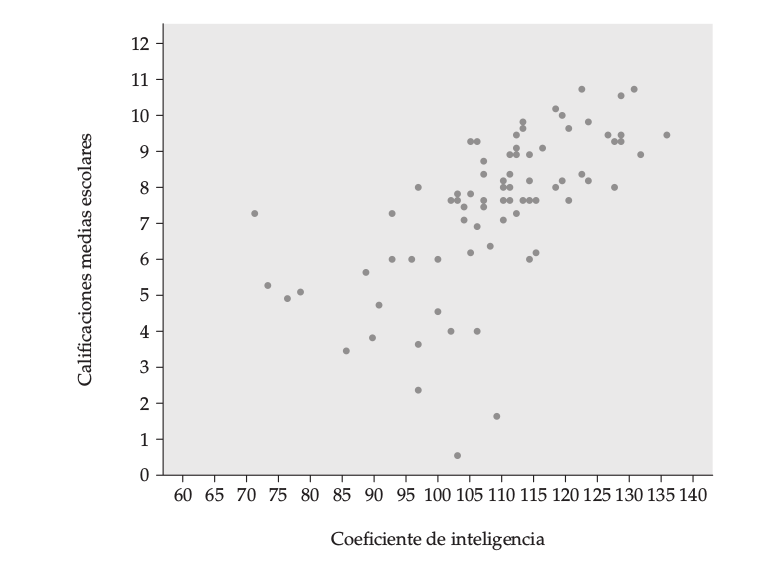
\includegraphics[scale=0.30]{imagen9.png}
\par\end{centering}
\caption{CI versus promedio }
\label{fig:fig8}
\end{figure}


\end{problema}

\begin{problema}
Un periódico universitario entrevista a un psicólogo a propósito de las evaluaciones que hacen los estudiantes de sus profesores. El psicólogo afirma: La evidencia demuestra que la correlación entre la capacidad investigadora de los profesores y la evaluación docente que hacen los estudiantes es próxima a cero. El titular del periódico dice: El profesor Cruz dice que los buenos investigadores tienden a ser malos profesores y viceversa. Explica por qué el titular del periódico no refleja el sentido de las palabras del profesor Cruz. Escribe en un lenguaje sencillo (no utilices la palabra “correlación”) lo que quería decir el profesor Cruz.

\end{problema}

%}

\end{document}
